\section{Implementation}
This system employs a technique called \textbf{deep metric learning} (i.e., deep-learning-based facial recognition)
to quantify the faces of students via dlib and face\_recognition module. In order to achieve facial
recognition in Python and OpenCV, I referenced the tutorial [1] on pyimagesearch by Adrian Rosebrock.
\newline

According to the tutorial [1], the network architecture for face recognition being used in this system
is based on ResNet-34 from the \textit {Deep Residual Learning for Image Recognition} paper [2] by Kaiming He,
Xiangyu Zhang, Shaoqing Ren and Jian Sun. The network in dlib was already trained by the creator of dlib,
Davis King, on a dataset of approximately three million images, while face\_recognition is a wrapper of
dlib which enables users to use it easily.
\newline

Users can manage their data, including courses, students and facial embeddings through GUI\@. They can also
initiate a roll call through GUI, letting students sign in to a class with facial recognition, as shown in
Figure 1.
\newline

\begin{figure}[b!]
  \centering
  \begin{subfigure}[b]{0.32\linewidth}
    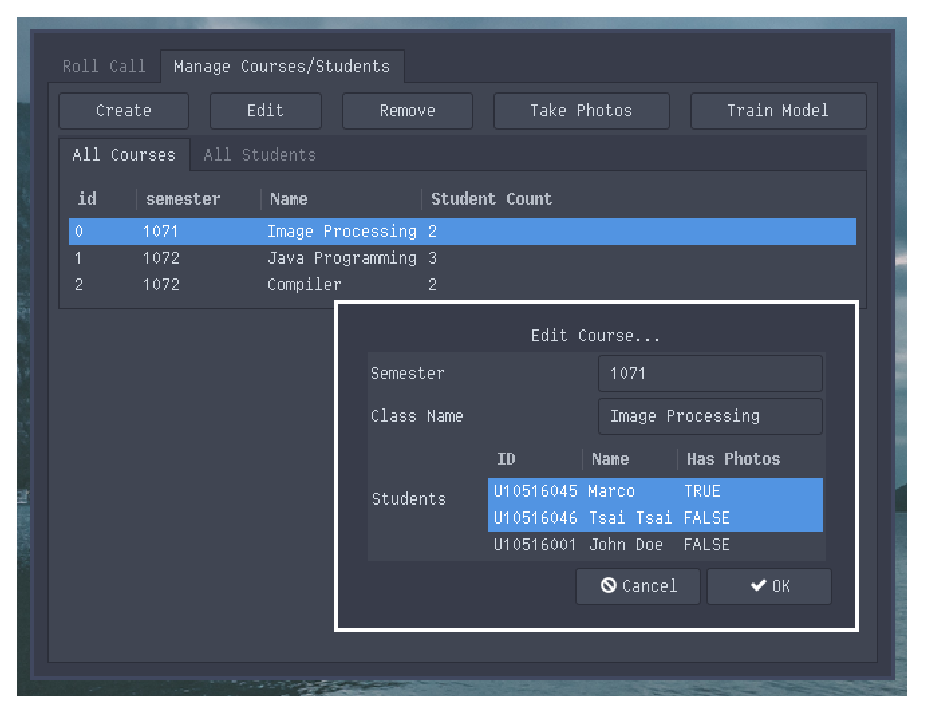
\includegraphics[width=\linewidth]{figures/preview1.eps}
    \caption{Managing courses.}
  \end{subfigure}
  \begin{subfigure}[b]{0.32\linewidth}
    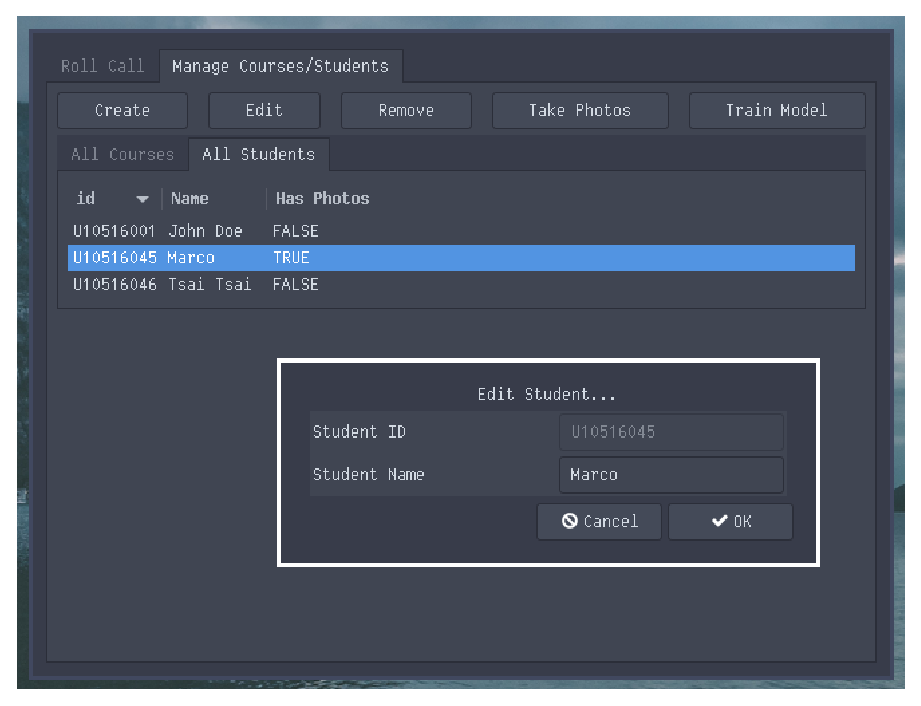
\includegraphics[width=\linewidth]{figures/preview2.eps}
    \caption{Managing students.}
  \end{subfigure}
  \begin{subfigure}[b]{0.32\linewidth}
    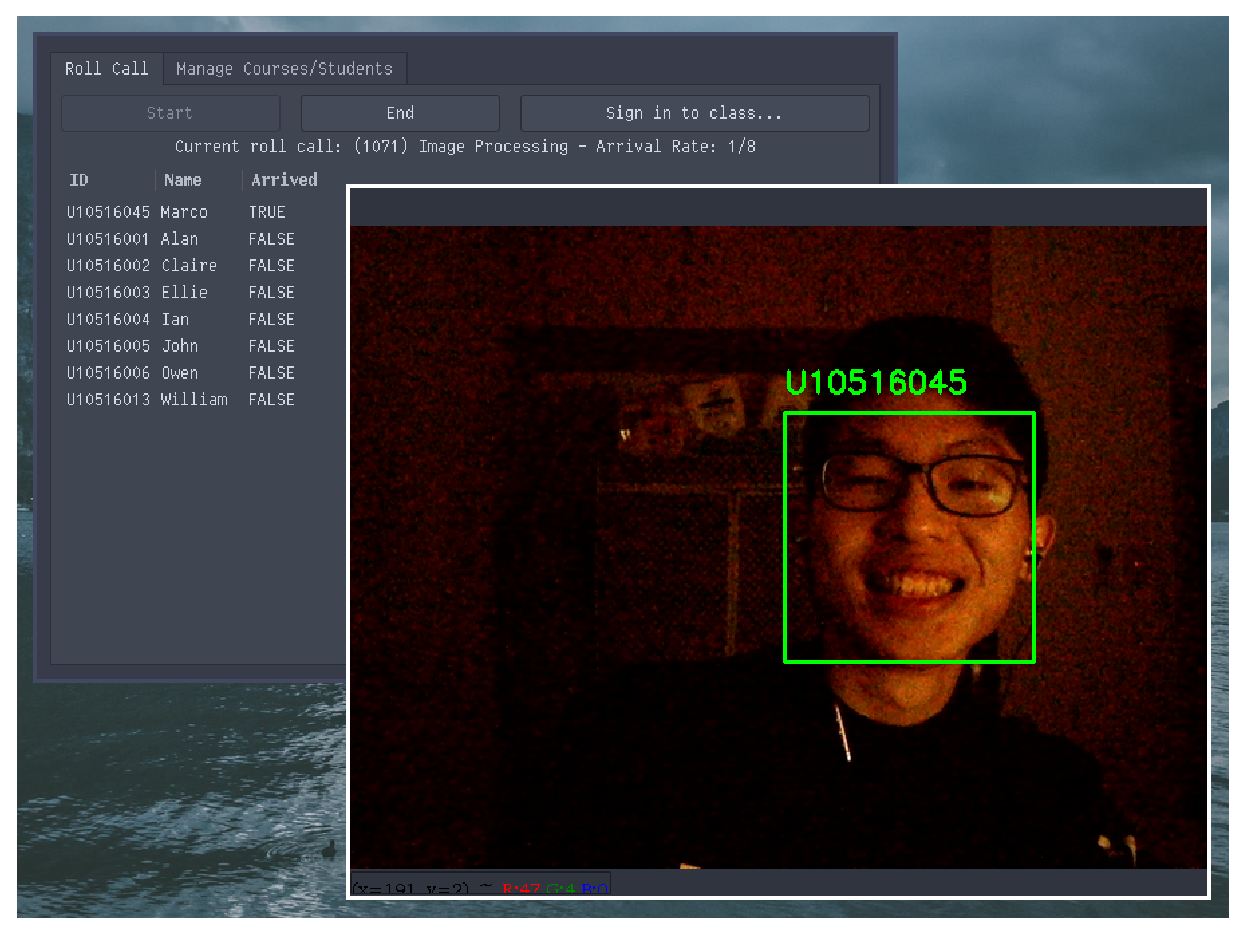
\includegraphics[width=\linewidth]{figures/preview3.eps}
    \caption{A student signing in.}
  \end{subfigure}
  \caption{pyRollCall's GUI, database and facial recognition.}
  \label{fig:implementation}
\end{figure}
